\chapter{The YodaQA System}
\label{ch:work}

My work on Question Answering so far has focused largely on building
a new open source QA platform that is sufficiently generic and modular,
features modern architecture and can serve both as scientific
research testbed and a practical system.
The outcome of this work is the \textbf{YodaQA} system.%
\footnote{Available open source at \url{https://github.com/brmson/yodaqa}
under the Apache Software Licence 2.0.}

\section{YodaQA Pipeline Architecture}
\label{sec:yodaqaarch}

The QA task is implemented in YodaQA as a pipeline that transforms the
question to a set of answers by applying a variety of analysis engines
and annotators.
It is composed from largely independent modules,
allowing easy extension with better algorithms
or novel approaches, while as a fundamental principle
all modules share a common end-to-end pipeline.
The pipeline is implemented in Java

The YodaQA pipeline is implemented mainly in Java,
using the Apache UIMA framework. \citep{UIMA}
YodaQA represents each artifact
as a separate UIMA CAS, allowing easy
parallelization and straightforward
leverage of pre-existing NLP UIMA components;
as a corollary, we compartmentalize
different tasks to interchangeable UIMA annotators.
Extensive support
tooling is included within the package.

The framework is split in several Java packages: \textbf{io} package takes care
of retrieving questions and returning answers, \textbf{pipeline} contains
classes of the general pipeline stages, \textbf{analysis} contains
algorithms for the particular analysis steps, \textbf{provider} has interfaces
to various external resources and \textbf{flow} carries UIMA helper classes
and a web interface dashboard.

\begin{figure}[hb]
\begin{center}
\resizebox{15cm}{!}{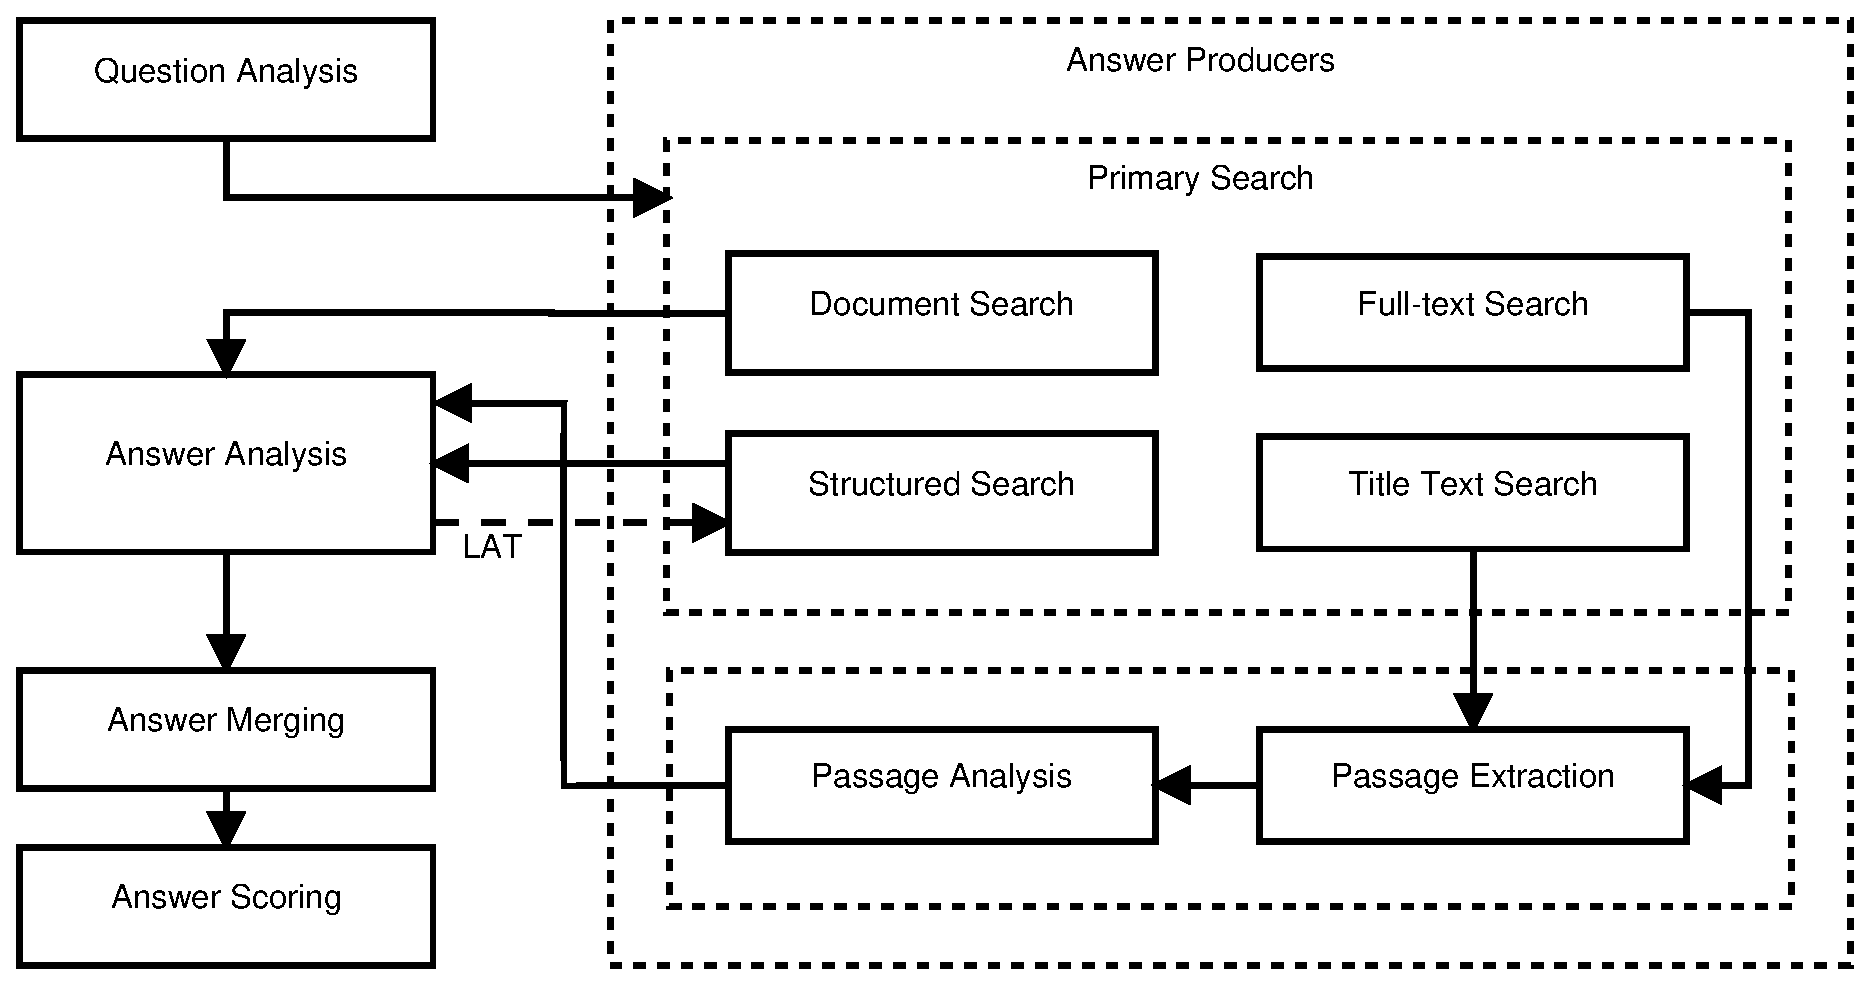
\includegraphics{yodaqa-arch.eps}}
%\vspace*{-0.75cm}
\caption{The general architecture of the YodaQA pipeline.  Present but unused final pipeline portions not shown.
TODO: Collapse answer production.  Plot sub-graphs with pipeline pieces in more detail.}
\label{fig:arch}
\end{center}
\end{figure}%\vspace{5mm}

The system maps an input question to ordered list of answer candidates in a pipeline fashion,
with the flow as in Fig.~\ref{fig:arch}, encompassing the following stages:

\begin{itemize}
\item \textbf{Question Analysis} extracts natural language features from
	the input and produces in-system representations of the question.
\item \textbf{Answer Production} generates a set of candidate answers based on the question,
	by performing a \textbf{Primary Search} in the knowledge bases according to the question clues
	and either directly using the results as candidate answers
	or selecting the relevant passages (the \textbf{Passage Extraction})
	and generate candidate answers from these (the \textbf{Passage Analysis}).
\item \textbf{Answer Analysis} generates answer features based on detailed analysis (most importantly, lexical type determination and coercion to question type).
\item \textbf{Answer Merging and Scoring} consolidates the set of answers, removing duplicates and using a machine learned classifier to score answers by their features.
\item \textbf{Successive Refining} (optional) prunes the set of questions in multiple phases, interjecting some extra tasks (evidence diffusion and gathering additional evidence).%
\footnote{We do not include Successive Refining in our evaluation or include further details as it is not beneficial in our current setup.}
\end{itemize}

The basic pipeline flow is much inspired by the Deep\-QA model
of IBM Watson \citep{WatsonPipeline}.  Throughout the flow, answer features
are gradually accumulated and some results of early flow stages (especially
the question analysis) are carried through the rest of the flow.


\section{YodaQA Reference Pipeline}
\label{sec:yodaqarefpip}

The reference pipeline currently considers an English-language task
as outlined in the Introduction --- answering open domain
factoid questions, producing a narrowly phrased answer.
We base the answers on information retrieval from both
unstructured (English Wikipedia --- \textit{enwiki})
and structured (DBpedia \citep{dbpedia}, Freebase \citep{freebase})
knowledge bases.

In our pipeline, we build on existing third-party NLP analysis tools,
in particular Stanford CoreNLP (Segmenter, POS-Tagger, Parser) \citep{StanfordCoreNLP} \citep{StanfordNNParser},
OpenNLP (Segmenter, NER) \citep{OpenNLP} and LanguageTool (Segmenter, Lemmatizer).%
\footnote{\url{http://www.languagetool.org/}}%
\footnote{Sometimes, different pipeline components default to different
NLP backends to perform the same task, e.g.\ segmentation,
based on empirically determined best fit.}
NLP analysis backends are freely interchangeable thanks
to the DKPro UIMA interface \citep{DKPro}.
For semantic analysis, we also rely heavily on the WordNet lexicon \citep{WordNet}.

Our key design rule is avoidance of hand-crafted rules and heuristics,
instead relying just on fully-learned universal mechanisms;
we use just about 10 hard-coded rules at this point, mostly
in question analysis.

For a practical illustration of the pipeline processing
two particular example questions,
see Appendix~\ref{app:analysis}.


\subsection{Question Analysis}

The question analysis involves
producing a part-of-speech tagging and dependency parse of the question text,
recognizing named entities and
performing entity linking%
\footnote{Right now, entities are linked just by an exact match of the main or alias label.}
to concepts (as represented by \textit{enwiki} articles).
The question representation we produce is similar in spirit
to DeepQA \cite{WatsonQuestion}: a bag-of-features including
a set of clues (keywords, keyphrases and linked concepts),
possible lexical answer types and the selection verb.

\textbf{Clues} represent keywords in the question that determine its content
and are used to query for candidate answers.
Clues based on different question components are assigned different weight
(used in search retrieval and passage extraction, determined empirically) ---
in ascending other, all noun phrases, noun tokens and the selection verb (SV);
the LAT (see below); named entities and matched concepts;
the question sentence subject (determined by dependency parse).

\textbf{Focus} is the center point of the question sentence
indicating the queried object.
Six simple hand-crafted heuristics extract the focus based on the dependency parse.
``name of ---'' constructions are traversed.

\textbf{LAT} (Lexical Answer Type) describes a type of the answer that would fit the question.
This type is not of a pre-defined category but may be an arbitrary English noun,
like in the DeepQA system. \citep{WatsonTyCor}
The LAT is derived from the focus, except question words are mapped to nouns
(``where'' to ``location'', etc.)
and adverbs (like ``hot'') are nominalized (to ``temperature'') using WordNet relations.

\textbf{SV} (Selection Verb) represents the coordinating verb of the
question that selects the answer with regard to other clues (like ``born'',
``received'', etc.)

\subsection{Unstructured Knowledge Bases}

The primary source of answers in our QA system is keyword search in free-text knowledge base
(the \textit{enwiki} in our default setting).
While the knowledge base has no formal structure,
we take advantage of the organization of the \textit{enwiki} corpus
where entity descriptions are stored in articles that bear the entity name as title
and the first sentence is typically an informative short description of the entity.
Our search strategies are analogous to basic DeepQA free-text information retrieval methods \citep{WatsonIR}.
We use the Apache Solr\footnote{\url{http://lucene.apache.org/solr/}} search engine (frontend to Apache Lucene).

\textbf{Title-in-clue search} \citep{WatsonIR} looks for the question clues in the article titles,
essentially aiming to find articles that describe the concepts touched in the question.
The first sentences of the top six articles (which we assume is its summary)
are then used in passage analysis (see below).

\textbf{Full-text search} \citep{WatsonIR} runs a full-text clue search in the article texts and titles,
considering the top six results.
The document texts are split to sentences which are treated as separate passages
and scored based on sum of weights of clues occuring in each passage\footnote{%
The \textit{about-clues} which occur in the document title have their weight divided by four (as determined empirically).}%
\footnote{We also carry an infrastructure for machine learning models scoring candidate passages,
		but they have not been improving performance so far.};
the top three passages from each document are picked for passage analysis.

\textbf{Document search} \citep{WatsonIR} runs a full-text clue search in the article texts;
top 20 article hits are then taken as potential responses,
represented as candidate answers by their titles.

\textbf{Concept search} retrieves articles that have been linked to entities mentioned in the question.
The first sentence as well as passages extracted like in the full-text search are used for passage analysis.

Given a picked passage, the \textbf{passage analysis} process executes an NLP pipeline and generates candidate answers;
currently, the answer extraction strategy entails simply converting all named entities and noun phrases to candidate answers.
Also, object constituents in sentences where subject is the question LAT are converted to candidate answers.

\subsection{Structured Knowledge Bases}

Aside of full-text search, we also employ structured knowledge bases organized in RDF triples;
in particular, we query the DBpedia \texttt{ontology} (curated) and \texttt{property} (raw infobox)
namespaces and the Freebase RDF dump.

For each concept
linked to an in-question entity, we query for predicates with this concept as a subject%
\footnote{All our knowledge bases are linked to \textit{enwiki}.}
and generate candidate answers for each object in such a triple, with the predicate label seeded as one LAT of the answer.

%For performance reasons, we limit the number of queried Freebase topics to 5 and retrieve only 40 properties per each;
%due to this limitation, we have manually compiled a blacklist of skipped
%``spammy'' properties based on past system behavior analysis
%(e.g.\ location's \textit{people\_born\_here} or music artist's \textit{track}).

Furthermore, we have trained a multi-label classifier (logistic regression)
that predicts \textit{property paths}
likely connecting an identified in-question concept with the answer in the knowledge base
graph based on particular forms in question representation. \cite{LeanFreebaseYao}
Unlike \cite{LeanFreebaseYao}, we consider long property paths as
Freebase is organized such that finding related concepts
often requires traversing intermediate nodes representing relationshibs (e.g.\ siblinghood).

\subsection{Answer Analysis}

In the answer analysis, the system takes a closer look at the answer snippet
and generates numerous features for each answer.
The dominant task here is type coercion,
i.e.\ checking whether the answer type matches the question LAT.

The answer LAT is produced by multiple strategies:
\begin{itemize}
	\item Answers generated by a named entity recognizer have LAT corresponding to the triggering model;
		we use stock OpenNLP NER models \textit{date}, \textit{location}, \textit{money}, \textit{organization}, \textit{percentage}, \textit{person} and \textit{time}.
	\item Answers containing a number have a generic \textit{quantity} LAT generated.
	\item Answer focuses (the parse tree roots) are looked up in WordNet and \textit{instance-of} pairs are used to generate LATs (e.g.\ \textit{Einstein} is \textit{instance-of} \textit{scientist}).
	\item Answer focuses are looked up in DBpedia and its ontology is used to generate LATs.
	\item Answers originating from a structured knowledge base carry the property name as an LAT.
\end{itemize}

Type coercion between question and answer LATs is performed using the WordNet
hypernymy relation --- i.e.\ \textit{scientist} may be generalized to \textit{person}, or \textit{length} to \textit{quantity}.
We term the type coercion score \textbf{WordNet specificity} and exponentially decrease it
with the number of hypernymy traversals required.
Answer LATs coming from named entity recognizer and quantity are not generalized.
We never generalize further once within the \texttt{noun.Tops} WordNet domain and
based on past behavior analysis, we have manually compiled a further blacklist
of WordNet synsets that are never accepted as coercing generalizations
(e.g. \textit{trait} or \textit{social group}).

The generated features describe the origin of the answer (data source, search result score, clues of which type matched in the passage, distance-based score of adjacent clue occurences, etc.), syntactic overlaps with question clues and type coercion scores (what kind of LATs have been generated, if any type coercion succeeded, what is the WordNet specificity and whether either LAT had to be generalized).

\subsection{Answer Merge-and-Score}

The merging and scoring process also basically follows a simplified DeepQA approach \citep{WatsonScoring}.
Candidate answers of the same text (up to basic normalization, like \textit{the-} removal) are merged;
element-wise maximum is taken as the resulting answer feature vector
(except for the \texttt{\#occurences} feature, where a sum is taken).
To reduce overfitting, too rare features are excluded
(when they occur in less than $1\%$ questions and $0.1\%$ answers).

Supplementary features are produced for each logical feature --- aside of the original value,
a binary feature denoting whether a feature has \textit{not} been generated
and a value normalized over the full set of answers
so that the distribution of the feature values over the answer
has mean 0 and standard deviation 1.
The extended feature vectors are converted to a score $s \in [0,1]$
using a logistic regression classifier.%
\footnote{An alternative gradient-boosted decision forest classifier is also
	available, but it is not beneficial in the default evaluation scenario yet.}
The weight vector is trained on the gold standard of a training dataset,
employing L2 regularization objective.  To strike a good precision-recall
balance, positive answers (which are about $p=0.03$ portion of the total)
are weighed by $0.5/p$.

\subsection{Successive Refining}

The pipeline contains support for additional refining and scoring phases.
By default, after initial answer scoring,
only the top 25 answers are kept with the intent of reducing noise for the next answer scoring classifier.
Answers are compared and those overlapping syntactically (prefix, suffix, or substring aligned with sub-phrase boundaries)
are subject to evidence diffusion where their scores are used as features of the overlapping answers.
Another answer scoring would be then performed, and the answer with the highest score is then finally output by the system.%
\footnote{There is also experimental support for additional evidence gathering phase, where the top 5 answers are looked up using the full-text search together with the question clues, and the number and score of hits are used as additional answer features and final answer rescoring is performed.  Nevertheless, we have not found this approach effective.}

However, while we have found these extra scoring steps beneficial with
weaker pipelines (in particular without the clue overlap features),
in the final pipeline configuration the re-scoring triggers significant
overfitting on the training set and we therefore ignore
the successive refining stage in the benchmarked pipeline.


\section{Performance Analysis}
\label{sec:results}

As we present performance analysis of our system,
we shall first detail our experimental setup;
this also includes discussion of our question dataset.

Then, we proceed with the actual results --- we measure the \textit{recall}
of the system (whether a correct answer has been generated and considered,
without regard to its score) and \textit{accuracy-at-one} (whether the
correct answer has been returned as the top answer by the system).
We find this preferrable to typical information retrieval measures like MRR or MAP
since in many applications, eventually only the single top answer output by the system
matters; however, we also show the \textit{mean reciprocial rank}
for each configuration and discuss the rank distribution of correct answers.

Aside of the performance of the default configuration, we also discuss
scaling of the system (extending the alotted answer time) and performance
impact of its various components (hold-out testing).

\subsection{Experimental Setup}

Our code is version tracked in a public GitHub repository
\url{https://github.com/brmson/yodaqa}, and the experiments presented
here are based on commit \texttt{TODO} (tagged as \texttt{v1.1}).
The quality of full-text search is co-determined by Solr version
(we use 4.6.0) and models of the various NLP components which are brought
in by DKPro version 1.7.0.
As for the knowledge bases, we use enwiki-20150112, DBpedia 2014,
Freebase RDF dump from Jan 11 2015, and WordNet 3.1.
Detailed instructions on setting up the same state locally (including
download of the particular dump versions and configuration files) are
distributed along the source code.

An automatic benchmark evaluation system is distributed as part of the
YodaQA software package.  The system evaluates the training and test questions
in parallel and re-trains the machine learning models before scoring the answers.
Therefore, in all the modified system versions considered below, a model trained
specifically for that version is used for scoring answers.

Our benchmark is influenced by two sources of noise.
First, the answer correctness is determined automatically by matching a predefined regex,
but this may yield both false positives and false negatives.%
\footnote{For example numerical quantities with varying formatting and units are notoriously tricky to match by a regular expression.}
Second, during training the models are randomly initialized and therefore their final
performance on a testing set flutters a little.

As a main benchmark of the system performance, we use a dataset of 430 training
and 430 testing open domain factoid questions.
(For system development, exclusively questions from the training set are used.)
This dataset is based on the public question answering benchmark from
the main tasks of the TREC 2001 and 2002 QA tracks
with regular expression answer patterns%
\footnote{\url{http://trec.nist.gov/data/qa/2001_qadata/main_task.html} and 2002 analogically.}
and extended by questions asked
to a YodaQA predecessor by internet users via an IRC interface.
This dataset was further manually reviewed by the author,
ambiguous or outdated questions were removed
and the regex patterns were updated based on current data.
We refer to the resulting 867 question dataset as \texttt{curated} and
randomly split it to the training and testing sets.\footnote{The remaining
7 questions are left unused for now.}

To further facilitate comparison of YodaQA to other systems,
we also benchmark its performance on the (i) original, unrevised and
unabridged TREC datasets
(even though the train/test splits might not be entirely compatible),
and (ii) the WebQuestions dataset \cite{WebQuestions}
(which represents several thousands of open domain factoid questions
tied to Freebase, popular as a semantic parsing benchmark).

\subsection{Benchmark Results}

TODO FIXME XXX

\begin{figure}[t]
% increase table row spacing, adjust to taste
\renewcommand{\arraystretch}{1.3}
\centering
\begin{tabular}{|c|cccc|}
\hline
Pipeline & Recall & Accuracy-at-1 & MRR & time \\ \hline \hline
default & 79.3\% & 32.6\% & 0.420 & 28.8s \\
% test  1119b6c 2015-03-09 Merge branch 'master... 144/289/430 33.5%/67.2% avgscore 0.504 mrr 0.424 avgtime 283643.667	+uv +uv
% test u1119b6c 2015-03-09 Merge branch 'master... 140/341/430 32.6%/79.3% avgscore 0.602 mrr 0.420 avgtime 283440.296
% test v1119b6c 2015-03-09 Merge branch 'master... 138/290/430 32.1%/67.4% avgscore 0.503 mrr 0.417 avgtime 283569.631
\hline
full-text scaling ($6\to12$ fetched results) & 82.3\% & 34.0\% & 0.430 & 50.0s \\
% test  e8e2f7b 2015-03-21 SolrFullPrimarySearc... 133/295/430 30.9%/68.6% avgscore 0.512 mrr 0.418 avgtime 12260.108	uv+ uv+
% test ue8e2f7b 2015-03-21 SolrFullPrimarySearc... 146/354/430 34.0%/82.3% avgscore 0.630 mrr 0.430 avgtime 11980.825
% test ve8e2f7b 2015-03-21 SolrFullPrimarySearc... 135/297/430 31.4%/69.1% avgscore 0.519 mrr 0.425 avgtime 12168.474

passage scaling ($3\to6$ picked passages) & 81.2\% & 31.4\% & 0.415 & 43.5s \\
% test  e1b3c91 2015-03-21 PassFilter: NUM_PICK... 137/296/430 31.9%/68.8% avgscore 0.509 mrr 0.419 avgtime 10368.150	v+u
% test ue1b3c91 2015-03-21 PassFilter: NUM_PICK... 135/349/430 31.4%/81.2% avgscore 0.616 mrr 0.415 avgtime 10088.654
% test ve1b3c91 2015-03-21 PassFilter: NUM_PICK... 146/294/430 34.0%/68.4% avgscore 0.516 mrr 0.432 avgtime 10275.724

document search scaling ($20\to40$) & 80.0\% & 31.6\% & 0.418 & 34.9s \\
% test  d8debbd 2015-03-21 SolrDocPrimarySearch... 135/292/430 31.4%/67.9% avgscore 0.499 mrr 0.410 avgtime 10859.761	u+v u+v
% test ud8debbd 2015-03-21 SolrDocPrimarySearch... 136/344/430 31.6%/80.0% avgscore 0.604 mrr 0.418 avgtime 10649.831
% test vd8debbd 2015-03-21 SolrDocPrimarySearch... 134/291/430 31.2%/67.7% avgscore 0.501 mrr 0.410 avgtime 10787.752

freebase scaling ($5\to10$ topics, $40\to80$ properties) & 79.8\% & 31.6\% & 0.416 & 29.8s \\
% test  6475b89 2015-03-22 FreebaseOntology: TO... 136/290/430 31.6%/67.4% avgscore 0.499 mrr 0.412 avgtime 6985.841
% test u6475b89 2015-03-22 FreebaseOntology: TO... 136/343/430 31.6%/79.8% avgscore 0.603 mrr 0.416 avgtime 6782.731
% test v6475b89 2015-03-22 FreebaseOntology: TO... 140/290/430 32.6%/67.4% avgscore 0.504 mrr 0.418 avgtime 6913.904

\hline
full-text hold-out & 49.5\% & 20.9\% & 0.277 & 5.8s \\
% test  cb27e81 2015-03-20 Merge branch 'master... 80/188/430 18.6%/43.7% avgscore 0.307 mrr 0.252 avgtime 1675.430	uv+
% test ucb27e81 2015-03-20 Merge branch 'master... 90/213/430 20.9%/49.5% avgscore 0.358 mrr 0.277 avgtime 1464.086
% test vcb27e81 2015-03-20 Merge branch 'master... 86/189/430 20.0%/44.0% avgscore 0.315 mrr 0.263 avgtime 1580.048

structured hold-out & 73.5\% & 29.1\% & 0.376 & 23.8s \\
% test  0659767 2015-03-20 YodaQA: Experimental... 113/265/430 26.3%/61.6% avgscore 0.448 mrr 0.362 avgtime 5443.057	uv+	vu+
% test u0659767 2015-03-20 YodaQA: Experimental... 125/316/430 29.1%/73.5% avgscore 0.546 mrr 0.376 avgtime 5261.876
% test v0659767 2015-03-20 YodaQA: Experimental... 125/267/430 29.1%/62.1% avgscore 0.461 mrr 0.380 avgtime 5371.852

type coercion hold-out & 79.3\% & 22.1\% & 0.314 & 30.0s \\
% test  a458fbf 2015-03-20 AnswerAnalysis: Expe... 90/246/430 20.9%/57.2% avgscore 0.388 mrr 0.304 avgtime 7249.693	uv+
% test ua458fbf 2015-03-20 AnswerAnalysis: Expe... 95/341/430 22.1%/79.3% avgscore 0.520 mrr 0.314 avgtime 7042.305
% test va458fbf 2015-03-20 AnswerAnalysis: Expe... 91/246/430 21.2%/57.2% avgscore 0.395 mrr 0.310 avgtime 7177.386

concept clues hold-out & 67.9\% & 23.0\% & 0.314 & 25.6s \\
% test  fdf189d 2015-03-20 QuestionAnalysis: Ex... 100/248/430 23.3%/57.7% avgscore 0.399 mrr 0.319 avgtime 6356.564	v+u
% test ufdf189d 2015-03-20 QuestionAnalysis: Ex... 99/292/430 23.0%/67.9% avgscore 0.490 mrr 0.314 avgtime 6104.581
% test vfdf189d 2015-03-20 QuestionAnalysis: Ex... 100/247/430 23.3%/57.4% avgscore 0.403 mrr 0.322 avgtime 6258.929

%external-resource LATs hold-out & 79.3\% & 22.1\% & 0.314 & 20.1s \\
% test  fe1b2e8 2015-03-20 AnswerAnalysis: Expe... 87/245/430 20.2%/57.0% avgscore 0.383 mrr 0.298 avgtime 5058.735	uv+
% test ufe1b2e8 2015-03-20 AnswerAnalysis: Expe... 95/341/430 22.1%/79.3% avgscore 0.520 mrr 0.314 avgtime 4888.693
% test vfe1b2e8 2015-03-20 AnswerAnalysis: Expe... 87/245/430 20.2%/57.0% avgscore 0.387 mrr 0.301 avgtime 4993.441

%fuzzy merging and evidence diffusion hold-out % & ...
% test  acbd992 2015-03-20 YodaQA pipeline: Exp... 129/290/430 30.0%/67.4% avgscore 0.497 mrr 0.405 avgtime 7364.049	uv+
% test uacbd992 2015-03-20 YodaQA pipeline: Exp... 139/341/430 32.3%/79.3% avgscore 0.602 mrr 0.420 avgtime 7131.604
% test vacbd992 2015-03-20 YodaQA pipeline: Exp... 135/290/430 31.4%/67.4% avgscore 0.503 mrr 0.413 avgtime 7276.565

clue overlap test hold-out & 79.3\% & 29.5\% & 0.390 & 30.1s \\
% test  65f5635 2015-03-20 AnswerAnalysis: Expe... 138/291/430 32.1%/67.7% avgscore 0.496 mrr 0.413 avgtime 7624.839	v+u
% test u65f5635 2015-03-20 AnswerAnalysis: Expe... 127/341/430 29.5%/79.3% avgscore 0.587 mrr 0.390 avgtime 7421.990
% test v65f5635 2015-03-20 AnswerAnalysis: Expe... 138/293/430 32.1%/68.1% avgscore 0.502 mrr 0.416 avgtime 7552.017
\hline
\end{tabular}
\vspace*{-0.2cm}
\caption{Benchmark results of various pipeline variants on the \textit{curated} test dataset.
MRR is the Mean Reciprocal Rank $|Q|\cdot\sum_{q\in Q}{1/r_q}$, time is the average time spent answering one question.}
\label{fig:bench}
\end{figure}

\begin{figure}[t]
\begin{center}
\resizebox{85mm}{!}{\includegraphics{ranks.eps}}
\vspace*{-0.75cm}
\caption{Number of questions $x$ that output the correct answer ranked at least $y$.}
\label{fig:ranks}
\end{center}
\end{figure}%\vspace{5mm}

Benchmark results over various pipeline configurations are laid out in Fig.~2. %\ref{fig:bench}.
Aside of the general performance of the system,
it is instructive to look at the histogram of answer ranks
for the default pipeline, shown in Fig.~\ref{fig:ranks}.
We can observe that while accuracy-at-one is 32.6\%,
accuracy-at-five is already at 52.7\% of test questions.

The information retrieval parameters of the default pipeline are selected so
that answering a question takes about 30s on average on a single core of
AMD FX-8350 with 24GB RAM and SSD backed databases.
(Note that no computation pre-processing was done on the knowledge bases or datasets;
bulk of the time per question is therefore spent querying the search engine and parsing sentences,
making it an accurate representation of time spent on previously unseen questions.)
By raising the limiting
parameters, we can observe further recall increase, and in case of considering
more full-text search results, also a solid accuracy improvement.  Our system
could therefore meaningfully make use of further computing resources.

We also benchmarked performance with various components of the pipeline
disabled.  We can see that the full-text and structured knowledge bases
are complementary to a degree, but the full-text base is eventually
a much stronger answer source for our system.  Type coercion and detection
of the concept clues in the question are both important heuristics for
our QA system.

Comparison of performance across multiple systems is currently non-trivial,
unfortunately, as there is no universally agreed experimental setup so far
and not even published results on the TREC datasets
from the years we use are readily available.
OpenEphyra seemed to typically achieve accuracy-at-one of ``above 25\%'' on
the TREC datasets including our years according to \citep{Ephyra2006}.
In the Answer Sentence Selection task \citep{WangQAGrammar},
Jacana and similar textual entaliement systems are reported%
\footnote{See the \textbf{ACL Wiki} topic \textit{Question Answering (State of the art)}.}
to achieve MRR around 0.750 but this task represents
a significant restriction upon the general end-to-end QA pipeline.

\section{System Performance}

In Fig.~\ref{fig:bench}, we compare various performance measures
with the most relevant previously published systems
(on the TREC dataset, as reported in the respective papers),
with ours benchmarked on non-curated version of the TREC 2002, 2003 dataset test split.

\begin{figure}[t]
%% increase table row spacing, adjust to taste
%\renewcommand{\arraystretch}{1.3}
\centering
\begin{tabular}{|c|cccc|}
\hline
System & Accuracy-at-1 & Recall & F1 & MRR \\ \hline
LLCpass03 \citep{LCC} (hand-crafted system) & 68.5\% & & & \\
AskMSR \citep{AskMSR} (web-search system) & 61.4\% & & & 0.507 \\ \hline
OpenEphyra \citep{Ephyra2006} (hand-crafted OSS) & ``above 25\%'' & & & \\
JacanaIR \citep{TreeEditIR2013Yao} (modern fully-learned OSS) & & & & 0.299$^*$ \\
OQA \citep{OQA} (modern fully-learned OSS) & & & 29\%$^{**}$ & \\ \hline
\textbf{YodaQA v1.0} & 25.1\% & 62.2\% & 35.8\% & 0.323 \\
\hline
\end{tabular}
\vspace*{-0.2cm}
\caption{Benchmark results of some relevant systems on the unmodified TREC dataset.\quad
$^*$ answer-bearing sentence retrieval\quad
$^{**}$ sub-sampled dataset with manual evaluation}
\label{fig:bench}
\end{figure}
